\documentclass{article}[12pt]

% Packages Petcu et al.
\usepackage[utf8]{inputenc} % allow utf-8 input
\usepackage{hyperref}       % hyperlinks
\usepackage{url}            % simple URL typesetting
\usepackage{booktabs}       % professional-quality tables
\usepackage{amsfonts}       % blackboard math symbols
\usepackage{nicefrac}       % compact symbols for 1/2, etc.
\usepackage{microtype}      % microtypography


\usepackage{algorithm}
\usepackage{algpseudocode}
\newif{\ifhidecomments}
\usepackage{enumerate}
\usepackage{wrapfig}
\usepackage{float}
\usepackage{amsmath}
\usepackage{multirow}
\usepackage{subcaption}
\usepackage{cleveref}

\usepackage{graphicx}
\usepackage{subcaption}
\usepackage[normalem]{ulem}


\usepackage{lipsum}
\usepackage{array}
\newcolumntype{C}[1]{>{\centering\arraybackslash}p{#1}}

\usepackage[multiple]{footmisc} % for two footnotes to to each other

\addbibresource{../journal/bibliography.bib} %Import the bibliography file
\usepackage[nonatbib, final]{neurips_2019}

\title{[Re] Privacy-preserving collaborative learning with automatic transformation search}

% The \author macro works with any number of authors. There are two commands
% used to separate the names and addresses of multiple authors: \And and \AND.
%
% Using \And between authors leaves it to LaTeX to determine where to break the
% lines. Using \AND forces a line break at that point. So, if LaTeX puts 3 of 4
% authors names on the first line, and the last on the second line, try using
% \AND instead of \And before the third author name.

%\author{%
%  Anonymous Author(s) \\
%  Affiliation\\
%  Address \\
%  \texttt{email} \\
%}

 \author{%
   Alfonso Taboada Warmerdam\\
   University of Amsterdam\\
   \texttt{alfonso.taboadawarmerdam@student.uva.nl} \\
   \And
   Lodewijk Loerakker \\
   University of Amsterdam\\
   \texttt{lodewijk.loerakker@student.uva.nl} \\
   % examples of more authors
   \And
   Lucas Meijer \\
   University of Amsterdam\\
   \texttt{lucas.meijer@student.uva.nl} \\
 %   \texttt{avtwarmerdam@gmail.com} \\
   \And
   Ole Nissen \\
   University of Amsterdam\\
   \texttt{ole.nissen@student.uva.nl} \\\\
 }

\begin{document}

\maketitle
\section*{Reproducibility Summary}

\subsection*{Scope of Reproducibility}

The authors introduce a novel approach to analyze Generative Adversarial Networks (GANs) and create interpretable controls for image manipulation and synthesis. This is done by identifying important latent directions based on Principal Component Analysis (PCA) applied either in the latent space or the feature space. We aim to validate the claims and reproduce the results of the original paper.

\subsection*{Methodology}

The code that was provided by the authors in Pytorch was reimplemented in Tensorflow 1.x for the pretrained StyleGAN and StyleGAN2 architectures. This was done with the help of the APIs provided by the original authors of these models.
\\
The experiments were run on a laptop with an Intel(R) Core(TM) i7-8750H CPU @ 2.20GHz processor, 16GB RAM, NVIDIA GeForce GTX 1060 with Max-Q Design (6GB VRAM) GPU, and Ubuntu 18.04.5 LTS.

\subsection*{Results}

We were able to reproduce the results and verify the claims made by the authors for the StyleGAN and StyleGAN2 models by recreating the modified images, given the seed and other configuration parameters.
Additionally, we also perform our own experiments to identify new edits and extend the truncation trick to images generated using StyleGAN.

\subsection*{What was easy}

The paper provides detailed explanations for the different mathematical concepts that were involved in the proposed method. This, augmented with a well-structured and documented code repository, allowed us to understand the major ideas in a relatively short period of time. Running the experiments using the original codebase was straightforward and highly efficient as well, as the authors have taken additional steps to employ batch processing wherever possible.

\subsection*{What was difficult}

Originally we were attempting to recreate identical images with zero delta in the RGB values. However, due to differences in the random number generators between PyTorch-CPU, PyTorch-GPU and Numpy, the random values were not the same even with the same seed. This resulted in minute differences in the background artifacts of the generated images. Additionally, there is a lack of open source Tensorflow 1.x APIs to access the intermediate layers of the BigGAN model. Due to time constraints, we were unable to implement these accessors and verify the images that the authors of GANSpace created using BigGAN.

\subsection*{Communication with original authors}

While conducting our experiments, we did not contact the original authors. The paper and codebase were organized well and aided us in effectively reproducing and validating the authors' claims.

\newpage

\section{Introduction}

A Generative Adversarial Network (GAN)\cite{gan} is a machine learning framework where two neural networks, the discriminator and the generator, compete with each other in a zero-sum game. The generator tries to trick the discriminator into believing that artificially generated samples belong to real data.

GANs have proven to be powerful image synthesis tools and are capable of producing high quality images. However, they provide little control over the features of the generated image. Existing solutions\cite{supervised} that add user control over the generated images require expensive supervised training on latent vectors.

GANSpace\cite{GANSpace} proposes a simple technique to discover interpretable GAN controls in an unsupervised manner. This is done by identifying important latent directions based on Principal Component Analysis (PCA) applied either on the latent space or the feature space. The author's experiments on StyleGAN\cite{stylegan}, StyleGAN2\cite{stylegan2} and BigGAN512-deep\cite{biggan} demonstrate that layer-wise decomposition of PCA directions leads to many interpretable controls, which affect both low and high level attributes of the output image.


\section{Scope of reproducibility}
\label{claims}


For our reproduction study, we aim to validate the effectiveness of the proposed technique in offering powerful interpretable controls on the output images in an unsupervised manner.

The following claims of the paper have been verified and tested successfully:
\begin{itemize}[noitemsep]
    \item PCA can be used to highlight important directions in the GAN's latent space.
    \item The GAN's output can be controlled easily in an unsupervised fashion.
    \item The earlier components control the higher-level aspects of an image, while the later directions primarily affect the minute details.
    \item Random directions do not yield meaningful decompositions as compared to the principal components identified using PCA.
\end{itemize}


\section{Methodology}

The principal components\cite{hotelling1933analysis} of a collection of points in real coordinate space are a sequence of $p$ unit vectors, where the $i^{th}$ vector is a direction of the line that best fits the data while being orthogonal to the remaining $i-1$ vectors. Principal Component Analysis (PCA) is an unsupervised algorithm used to compute the principal components and perform a change of basis of the data using one or more of the computed components, increasing the interpretability of the data while minimizing its information loss\cite{jolliffe2016principal}. It is commonly used in exploratory data analysis and for dimensionality reduction when dealing with high-dimensional noisy data. The authors of GANSpace propose a technique for identifying interpretable controls in an unsupervised fashion on pretrained GANs using PCA. Specifically, they show that layer-wise perturbations along the principal components generated using PCA on the latent space of StyleGAN based networks can be used to generate human-interpretable transformations on the synthesized images.

Mathematically, a GAN can be expressed as a neural network $G(\mathbf{z})$ that generates an image $I: \mathbf{z} \sim p(\mathbf{z}), I = G(\mathbf{z})$. Here, $p(\mathbf{z})$ is a probability distribution from which the latent vector $\mathbf{z}$ is sampled. The network $G(\mathbf{z})$ can be further decomposed into $L$ intermediate layers $G_1\ldots G_L$. In the StyleGAN/StyleGAN2 models, the input to the first layer is a constant $\mathbf{y}_0$. The output and input to the remaining layers is computed as:

\begin{equation}
  y_i = G_i(y_{i-1}, \mathbf{w}),\text{ where }\mathbf{w} = M(\mathbf{z})
\end{equation}

$M$ is a an $8$-layer multilayer perceptron which is a non-linear function of $\mathbf{z}$. The number of layers $L$ depends on the resolution of the generated image. At each layer, the generated image is upsampled by a factor of $2$.

\begin{figure}[H]
  \centering
  \includegraphics[scale=0.25]{figs/stylegan.png}
  \caption{Architecture of StyleGAN\cite{stylegan}}
  \label{fig:stylegan}
\end{figure}

\begin{figure}[H]
  \centering
  \includegraphics[width=\textwidth]{figs/stylegan2.png}
  \caption{Architecture of StyleGAN2\cite{stylegan2}}
  \label{fig:stylegan2}
\end{figure}

The images generated by StyleGAN and StyleGAN2 can be controlled by identifying the principal axes of $p(\mathbf{w})$, which is the probability distribution of the output of the mapping network $M$. First, we sample $N$ latent vectors $\mathbf{z}_{1:N}$ and compute the corresponding $\mathbf{w}_{i} = M(\mathbf{z}_{i})$. The PCA of these $\mathbf{w}_{1:N}$ values gives us the basis $\mathbf{V}$ for $\mathcal{W}$. The output attributes of a new image given by $\mathbf{w}$ can then be controlled by varying the PCA coordinates of $\mathbf{x}$ before feeding them into the synthesis network:

\begin{equation}
    \mathbf{w'} = \mathbf{w} + \mathbf{Vx}
\end{equation}

Each entry $x_{k}$ of $\mathbf{x}$ is a separate control parameter which can be modified to update the desired attributes of the output image.

We follow the same notation used by the authors to denote edit directions in this report. $E(\mathbf{v}_{i}, j-k)$ means moving along component $\mathbf{v}_{i}$ from layers $j$ to $k$. Identifying specific edits, for example "changing the color of a car", is done via exploratory analysis using a trial-and-error method. The authors have created a GUI-based application for this purpose.

\subsection{Model descriptions}

We use NVIDIA's official implementation of StyleGAN\footnote{\url{https://github.com/NVlabs/stylegan}} and StyleGAN2\footnote{\url{https://github.com/NVlabs/stylegan2}} models.
The original code uses a PyTorch/NumPy implementation of StyleGAN and StyleGAN2 which creates a PyTorch model and copies the weights from NVLabs' implementations which are in Tensorflow. However, we directly use the NVLabs' APIs with NumPy and make changes to the official GANSpace codebase to support the same.

\subsection{Datasets}

The experiments in the paper were performed using the FFHQ, LSUN Car, CelebA-HQ, Wikiart, Horse and Cat datasets. The official Tensorflow implementation of StyleGAN contains links to download pretrained models on FFHQ, LSUN Car, Wikiart, Horse and Cat. The models trained on Wikiart were downloaded from awesome-pretrained-stylegan\footnote{\url{https://github.com/justinpinkney/awesome-pretrained-stylegan}}.

In addition to the datasets used by the authors, we also perform our own experiments on the Beetles dataset which was downloaded from awesome-pretrained-stylegan2\footnote{\url{https://github.com/justinpinkney/awesome-pretrained-stylegan2}}.


\subsection{Experimental setup}

All the experiments were conducted on a laptop with an Intel(R) Core(TM) i7-8750H CPU @ 2.20GHz processor, 16GB RAM, NVIDIA GeForce GTX 1060 with Max-Q Design (6GB VRAM) GPU, and Ubuntu 18.04.5 LTS. The generated images from our experiments were evaluated visually to determine whether the edits were working as expected.

\section{Results}

We were able to reproduce the results and verify the claims (mentioned in Section \ref{claims}) made by the authors for the StyleGAN and StyleGAN2 models by recreating the modified images, given the configuration parameters. Additionally, we also perform our own experiments to provide additional results that validate the effectiveness of the technique employed by GANSpace.


\subsection{Effectiveness of PCA}

\begin{figure}[H]
    \centering
    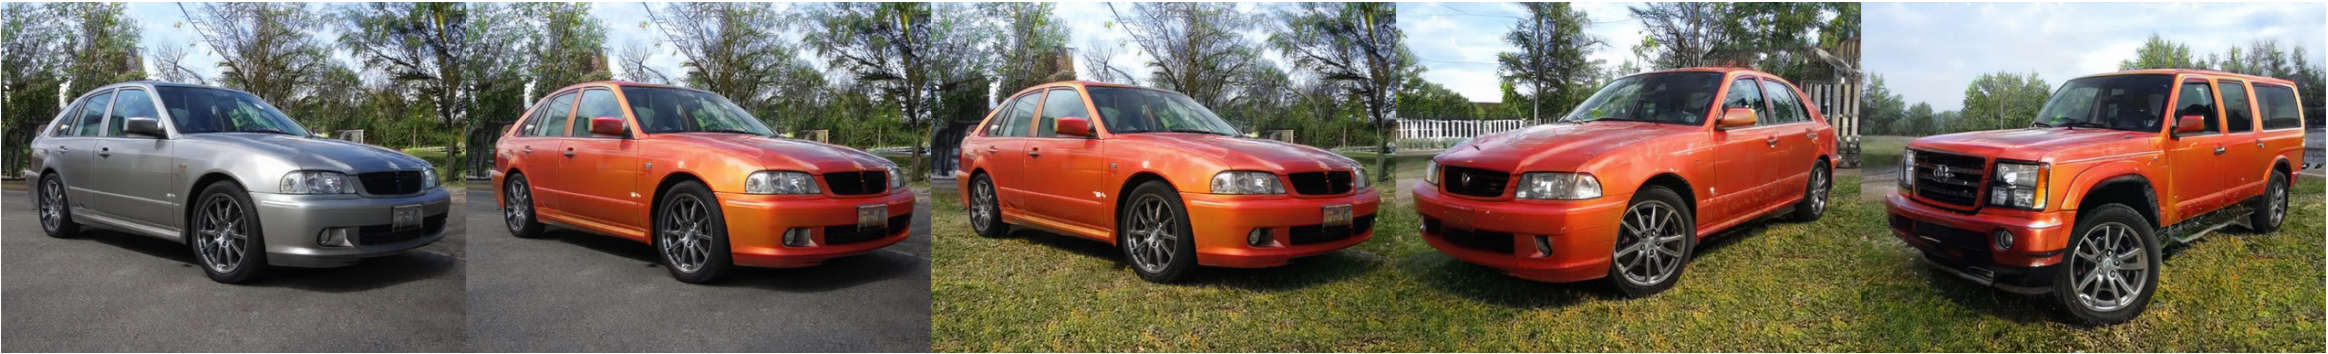
\includegraphics[width=\textwidth]{figs/figure1_StyleGAN2_cars.png}
    \caption{Sequences of image edits performed using control discovered with StyleGAN2 cars: ``Initial Image" $\rightarrow$ ``Change Color" $\rightarrow$ ``Add Grass" $\rightarrow$ ``Rotate" $\rightarrow$ "Change Type"}
    \label{fig:cars}
\end{figure}

Figure \ref{fig:cars} highlights the effectiveness of PCA on changing the low and high level attributes of the image. We are able to control object shape, colour and pose as well as nuanced landscape attributes.

The edit directions corresponding to each of the edits are: $E(\mathbf{v}_{22}, 9-10)$ ("Change Color"), $E(\mathbf{v}_{11}, 9-10)$ ("Add Grass"), $E(\mathbf{v}_{0}, 0-4)$ ("Rotate") and $E(\mathbf{v}_{16}, 3-5)$ ("Change type").

\subsection{Unsupervised vs. Supervised methods}

\begin{figure}[H]

  \subfloat[Edit directions identified by PCA ($E(\mathbf{v}_{1}, 0-1)$)]{%
    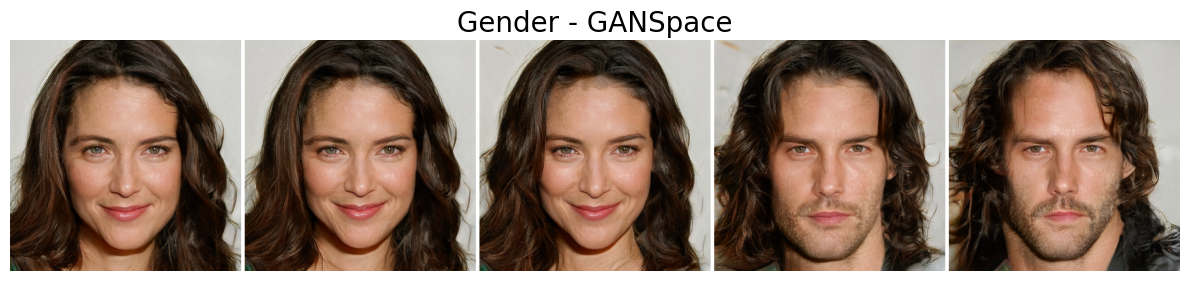
\includegraphics[clip,width=\columnwidth]{figs/figure5_Gender-GANSpace_scale=-3dot2.png}
  }

  \subfloat[Edit directions identified by supervised methods\cite{supervised}]{%
    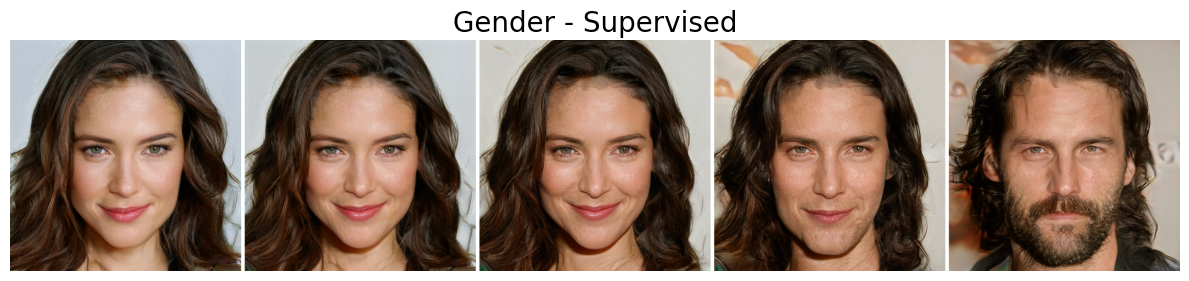
\includegraphics[clip,width=\columnwidth]{figs/figure5_Gender-Supervised_scale=1dot2.png}
  }
  
  \caption{Comparison of edits using unsupervised and supervised methods}
  \label{fig:faces}
\end{figure}

Previous methods for finding interpretable directions in GAN latent spaces require external supervision, such as labeled training images or pretrained classifiers. GANSpace, on the other hand, automatically identifies variations intrinsic to the model without supervision. This has been validated using the CelebA-HQ Faces dataset by comparing the edit directions found through PCA to those found in previous works using supervised methods.

Figure \ref{fig:faces} shows that comparable edits can be obtained in a completely unsupervised fashion. Additionally, GANSpace can be used to identify new edits which have not been previously demonstrated. Supervised methods are not viable for this task as supervising each new edit would be costly. It is also difficult to know in advance which edits are even possible in supervised approaches.

\subsection{PCA components vs. Random directions}

\begin{figure}[H]
    \centering
    \includegraphics[width=\textwidth]{figs/cats.png}
    \caption{Illustration of the significance of the principal components as compared to random directions in the intermediate latent space of StyleGAN2.}
    \label{fig:cats}
\end{figure}

The original authors claim that the earlier PCA components primarily control the geometry and other high-level aspects (pose and style), while the lower components capture minute details. Additionally, they claim that fixing and randomizing randomly-chosen directions do not yield PCA-like meaningful decompositions, thus showing the importance of identifying good directions using PCA. This has been illustrated in Figure \ref{fig:cats}, where different subsets of principal coordinates and random coordinates are randomized while keeping the latent vector constant. In Figure \ref{fig:cats}a, the first eight principal coordinates $\mathbf{x}_{0:7}$ are fixed and the remaining $504$ coordinates $\mathbf{x}_{8:512}$ are randomized. This changes the background and appearance of the cat while keeping the cat's pose and camera angle constant. Conversely, Figure \ref{fig:cats}b shows that fixing the last $504$ coordinates and randomizing the first eight yields images where the camera and orientation vary, but the color and appearance are held roughly constant. Figure \ref{fig:cats}c and Figure \ref{fig:cats}d shows the results of the same process applied to random directions. The images illustrate that any given $8$ directions have no distinctive effect on the output.

\subsection{Additional results not present in the original paper}

\subsubsection{New edits}

We identify new edits on the Stylegan2 Beetles dataset. Edit $E(\mathbf{v}_{2}, 0-17)$, referred to as "Patterns", adds a pattern on the shell of the beetle as well as increasing the overall size of the beetle. The generated pattern varies depending on the seed used to sample $\mathbf{w}$.

\begin{figure}[H]

\subfloat[Beetle generated with seed 1819967864]{%
  \includegraphics[clip,width=\columnwidth]{figs/figure7_beetles_pattern.png}%
}

\subfloat[Beetle generated with seed 1]{%
  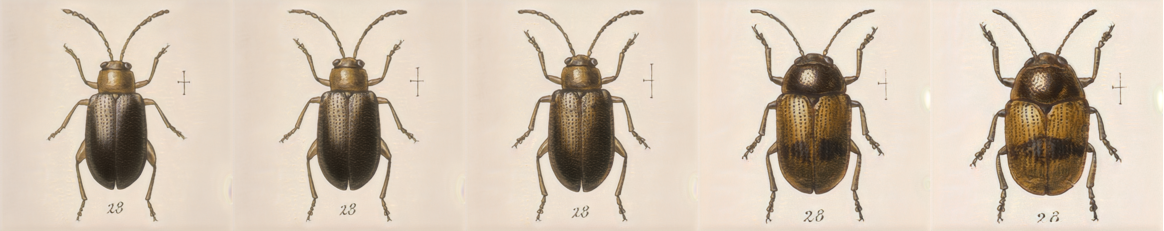
\includegraphics[clip,width=\columnwidth]{figs/figure7_different_beetle_pattern.png}%
}

\caption{"Patterns" edit applied on the output images of StyleGAN2 Beetles}

\end{figure}

\subsubsection{Truncation Trick on StyleGAN}

The "Truncation Trick" is a procedure applied to the latent vectors to improve the quality of the generated images at the expense of variety in the images. It does this by sampling the latent vectors from a truncated distribution that is closer to the average of the latent vectors sampled during training, thereby reducing the variance of the latent vectors used during inference. The authors of \cite{biggan} show that using the truncation trick improves the Fréchet Inception Distance (FID) and Inception Score (IS).

In the StyleGAN/StyleGAN2 models, the truncation trick is applied on the latent space $\mathbf{w}$, which is the output of the mapping network $M$. During the training process, a running average $\mathbf{w}_{avg}$ of the latents is computed. Later, the latents sampled during inference are truncated to lie close to $\mathbf{w}_{avg}$. Equation~\ref{eq:2} shows the truncation process on StyleGAN/StyleGAN2 models:

\begin{equation}
    \mathbf{w'} = \mathbf{w}_{avg} + \psi (\mathbf{w} - \mathbf{w}_{avg})
    \label{eq:2}
\end{equation}

During our experiments, we noticed that the original authors use the truncation trick on images generated using StyleGAN2 to reduce the number of artifacts. However, this is not enabled for StyleGAN images. We found that enabling truncation while applying edits on StyleGAN images improved their quality as well. We demonstrate this using the Wikiart dataset through the "Head Rotation" ($E(\mathbf{v}_{7}, 0-1)$) and "Simple Strokes" ($E(\mathbf{v}_{9}, 8-14)$ edits. In Figure~\ref{fig:truncation_psi}, we can see that the generated faces contain less noise and artifacts when the truncation trick is used. For example, the lower half of the person's face in the "Head Rotation" image does not contain as much noise as their counterpart which does not employ the truncation trick. Here, we can also observe the change in the generated images as truncation psi is decreased a lower value of $0.25$. This truncates the sampled latents to lie very close to the average and results in images that look very similar to each other. If truncation psi is set to $0$, then according to Equation~\ref{eq:2}, we can see that the truncated latent $\mathbf{w}'$ is always equal to $\mathbf{w}_{avg}$.

\begin{figure}

\subfloat["Head Rotation" and "Simple Strokes" edits on StyleGAN Wikiart with truncation psi set to 0.25]{%
  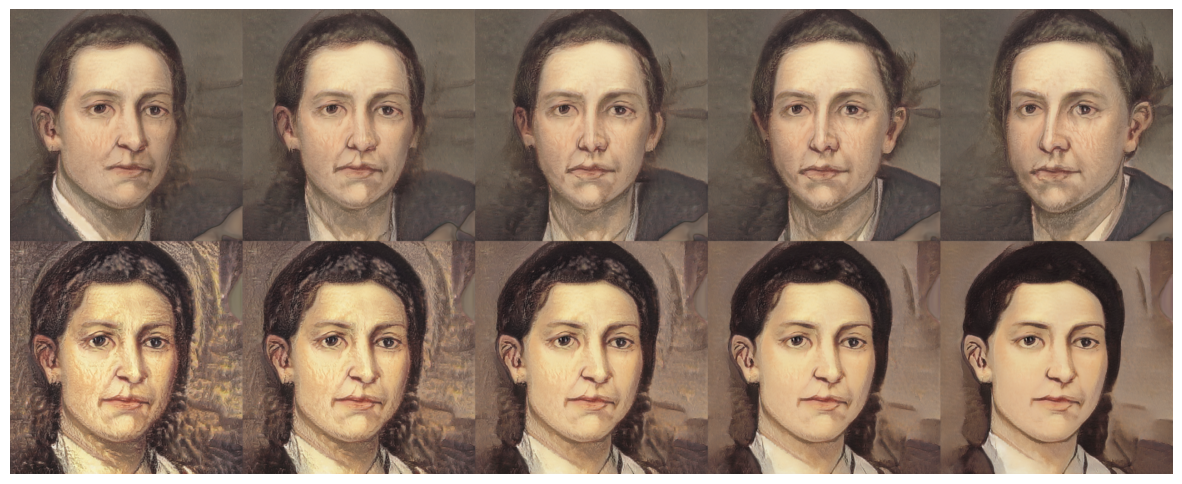
\includegraphics[clip,width=\columnwidth]{figs/wikiart_truncation_psi_0dot25.png}
}

\subfloat["Head Rotation" and "Simple Strokes" edits on StyleGAN Wikiart with truncation psi set to 0.7]{%
  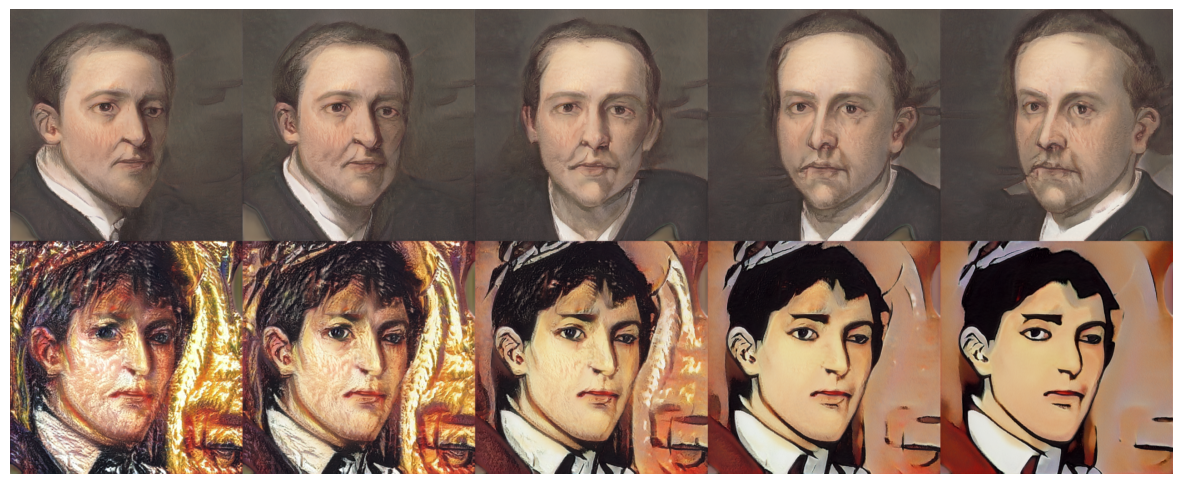
\includegraphics[clip,width=\columnwidth]{figs/wikiart_truncation_psi_0dot7.png}
}

\subfloat["Head Rotation" and "Simple Strokes" edits on StyleGAN Wikiart without truncation psi]{%
  \includegraphics[clip,width=\columnwidth]{figs/wikiart_truncation_psi_1dot0.png}%
}

\caption{Quality of images generated by StyleGAN before and after applying the "truncation trick".}
\label{fig:truncation_psi}
\end{figure}

\section{Discussion}

After performing our experiments, we feel that the results justify the claims of the paper. This is further bolstered by the fact that the proposed method worked on different datasets which were not covered by the original authors.

\subsection{What was easy}

The paper provides detailed explanations for the different mathematical concepts that were involved in the proposed method. This, augmented with a well-structured and documented code repository, allowed us to understand and verify the major ideas in a relatively short period of time. Additionally, the paper provided a lot of examples on various datasets to demonstrate exactly how their algorithm works. The authors ensured that all the figures in the paper had accompanying code to recreate them.

NVIDIA's implementation of StyleGAN and StyleGAN2 provided access to well written API's which we could integrate easily into the author's codebase.

\subsection{What was difficult}

While running our experiments, we noticed that there was a small difference in the RGB values of the recreated images. This was due to the difference in the random values generated by PyTorch-CPU, PyTorch-GPU and Numpy random number generators even when seeded with the same seed. The noise variables in the StyleGAN networks were not identical because of this. This resulted in minute differences in background artifacts of the images.

\begin{table}[H]
\centering
\begin{tabular}{cc}
\hline
Python Library & Random Number \\ \hline
PyTorch 1.3.1 (CPU)     & 0.3367                 \\
PyTorch 1.3.1 (GPU)     & 0.1940                 \\ 
Numpy 1.20.1            & 0.49671415             \\ \hline
\end{tabular}
\caption{Random values generated using different Python libraries seeded with 42}
\end{table}

We were not able to replicate the author's experiments on BigGAN512-deep due to time constraints. 

\subsection{Communication with original authors}

While conducting our experiments, we did not contact the original authors. The paper and codebase were organized well and aided us in effectively reproducing and validating the authors' claims.

\setlength\bibitemsep{0pt}
\printbibliography

\newpage

\appendix
\section*{Appendix}


\section{Counterfactual Generative Network Architecture} \label{sec:cgn-architecture}
In \cref{fig:cgn-architecture}, we provide an overview of the architecture of the CGN as provided in the paper. It illustrates how the CGN is split into four mechanism: the shape mechanism, the texture mechanism, the background mechanism, and the composer. Each mechanism takes a noise vector $\v u$ and a label $y$ as input. To generate a counterfactual image, we sample $\v u$ and then sample a separate $\v y$ for each mechanism \citewithauthor{Sauer2021ICLR}.

\begin{figure}[H]
    \centering
    \includegraphics[width=0.9\linewidth]{../openreview/media/cgn-architecture.pdf}
    \caption{\textbf{CGN architecture.} Components with \textcolor{Blue}{trainable parameters are blue}, components with \textcolor{Green}{fixed parameters are green} \cite{Sauer2021ICLR}. The dotted lines indicate that the cGAN is only used for training \cite{Sauer2021ICLR}.}
    \label{fig:cgn-architecture}
\end{figure}


% Can you guys come up with other suggestions?
\section{Counterfactual images and explainability in artificial intelligence} \label{sec:counterfactuals}
One of the primary contributions of the work by \citewithauthor{Sauer2021ICLR} is the proposed method to create high-quality `counterfactual' images, which can be used to make a classifier more robust to spurious signals. As the concept of \emph{counterfactual explanations} is closely related to the idea of explainable artificial intelligence (XAI) but is never explicitly mentioned in the paper, we first want to place the article in a broader context to achieve a deeper understanding of how the considered work relates to other developments within this field of research \cite{arrieta2020explainable}.

Based on the review by \citewithauthor{verma2020counterfactual}, approaches for explainability in machine learning can be roughly divided into one of two categories:
(i) methods that use inherently interpretable and transparent models, and (ii) methods that generate post-hoc explanations for opaque models.

% \begin{enumerate*}[(i)]
%     \item methods that use inherently interpretable and transparent models, and
%     \item methods that generate post-hoc explanations for opaque models.
% \end{enumerate*}
The idea of counterfactual explanations belongs to the example-based approaches within the category of post-hoc explanations, that seek to offer explanations by either providing datapoints that receive the same prediction label as the observed datapoint, or by providing datapoints whose prediction label is different from the observed datapoint.

Consider the example where a classifier is trained to distinguish images from polar bears and American black bears. Given an image that has been classified by the model as a black bear, we could attempt to provide a post-hoc explanation for the model's prediction using a visual counterfactual explanation (i.e., a modified version of the input image that would be classified as a polar bear instead). These explanations can, for example, be generated using techniques such as StylEx \cite{lang2021explaining}. A reasonable visual counterfactual explanation could consist of the input image, modified such that the fur of the black bear is now colored white. However, as most images of polar bears have a snow-background, and most images of American black bears likely do not, it is possible that the suggested visual counterfactual explanation still contains a black bear, but now on a snowy background.

In this case, one could argue that the background-explanation that is captured by the model is a spurious signal. That is, the classifier `falsely' makes predictions on the background, even though the background, in reality, does not affect the actual object itself. Although this spurious signal might seem innocent within the context of this example, other spurious signals can play a role in a variety of high stake deep learning applications, such as AI in medical-imaging \cite{degrave2021ai} and networks trained for military purposes \cite{guidotti2018survey}. While counterfactual explanations are thus capable of \emph{revealing} such spurious signals, the proposed method using counterfactual images by \citeauthor{Sauer2021ICLR} provides an approach to \emph{mitigate} this effect.


\section{Improved CGN Training for MNIST} \label{sec:edge_loss_appendix}
% For the reproducibility study, we tried training the CGN on the MNISTS and a classifier with the generated images. However, a problem was encountered that was not described by Sauer et al. \cite{Sauer2021ICLR}. The accuracy of the classifier was very low, and wildly varied per run of the CGN training. It ranged between 30\% and 80\%.

While training the CGN on the MNIST, we encountered an issue that was not mentioned in the original paper. During the training process, we observed that while some digits were captured almost perfectly by the model, other digit masks seemed to collapse to a state where there was a black circular shape in the center of the image with a surrounding white border (see \cref{fig:mnist-failed-samples}). When using the generated counterfactual datasets from these imperfect models to train a classifier, we then observed that the number of `correct' (i.e., non-collapsed) images correlated strongly with the classifier performance.


% That is, if 7 out of 10 digits did not collapse to the erroneous state, the classifier would achieve a test accuracy around 70\%. The number of `broken' digits seemed to vary considerably, resulting in test accuracies ranging between 20\% and 70\% while using the exact same experimental setup. Running the experiment multiple times seemed to indicate that every digit had a 50\% change of `breaking' at the start of the training process (\cref{fig:mnist-failed-samples}). Since the authors reported a test accuracy above 90\% for the Colored MNIST dataset and each digit would only have a 50\% chance of training properly when running the model, this would mean we would theoretically need to retrain the model $1/0.5^{10}=1024$ times in order to ensure that we achieve the same model performance.

% As retraining the model 1024 times was not feasible, we have attempted to find a solution to make the training process for the MNIST datasets more consistent.
% Since the problem with broken digits seems to occur because the model produces the foreground near the edges and the background in the center, our initial attempt to solve the issue was to use different $\lambda$-hyperparameters for the losses, to ensure that the authors did not unintentionally provide incorrect $\lambda$-values. However, as the $\lambda$-description from the original paper did not directly match with the $\lambda$-parameters in the code implementation, it was not clear which parameters correspond to which $\lambda$-values. Therefore, we propose our own solution based on the observation that the model produces a foreground near the edges, even though MNIST digits are always located in the center.

% To solve this, we performed a qualitative analysis of the generated images for (single-)colored MNIST, where this problem is most prevalent. Some samples are shown in \cref{fig:mnist-failed-samples}. It appears that there is about a 50\% probability per digit that the network producing the fore-/background mask gets stuck in producing a foreground near the edges, and a background in the center. This is clearly problematic as the foreground containing the digit should be in the center.

% *** OLD EDGE LOSS EXPLANATION FROM HERE ***
% This observation inspired a solution where we add an extra loss term that encourages the center of the mask to be foreground and the edges background. Let us define the edge region $\mathcal{E}$ as the set of pixels that are within $s$ pixels of an edge. The center region $\mathcal{C}$ then contains the remaining pixels and forms a square of $w - 2s$ by $h - 2s$ pixels, where $h$ is the height and $w$ the width.
% % Taking this into account,
% Considering this,
% we optimize the shape mechanism by adding the center loss to
% shape loss:
% % $\mathcal{L}_{\text{shape}}$:
% \begin{equation} \label{eq:center-loss}
%     \mathcal{L}_{center}(\v m) = \mathbb{E}_{p(\v u, y)} \left[\frac{1}{N} \sum_{i=1}^N m_i \cdot \left([i \in \mathcal{E}] - [i \in \mathcal{C}]\right)\right].
% \end{equation}
% Recall that mask values close to 1 correspond to foreground pixels, and mask values close to 0 to background pixels. As a result, adding this loss encourages the foreground to consistently be in the center. As shown in \cref{fig:mnist-failed-samples} and \cref{fig:mnist-improvements}, this greatly reduces the frequency of this problem. Averaged over 47 runs without the extra loss and 20 runs with the extra loss, it increased the frequency of non-broken images from 56\% to 89\% when the loss weight was 0.1 and $s = \lfloor \frac15 w \rfloor = 5$.
% *** TO HERE ***



% *** NEW EDGE LOSS EXPLANATION FROM HERE (PAUL) ***
Any attempt to remedy this issue using adjusted hyperparameter configurations proved to be ineffective, because the hyperparameter names in the provided default configuration-files did not directly correspond to the descriptions given in the original paper.
This observation inspired a solution where we add an extra loss term to the training objective, which penalizes mask-pixels at the borders of the image. Specifically, if we define the edge region $\mathcal{E}$ as the set of pixels that are within $s$ pixels from the edge, the edge loss function can be defined as the sum of all pixel values $m_i$ within the specified edge region:
% $\mathcal{L}_{\text{shape}}$:
\begin{equation} \label{eq:center-loss}
    \mathcal{L}_{edge}(\v m) = \mathbb{E}_{p(\v u, y)} \left[\frac{1}{N} \sum_{i=1}^N m_i \cdot  [i \in \mathcal{E}]\right],
\end{equation}
% \begin{equation} \label{eq:center-loss}
%     \mathcal{L}_{edge}(\v m) = \mathbb{E}_{p(\v u, y)} \left[\frac{1}{N} \sum_{x \in \mathcal{E}} x\right],
% \end{equation}
where $N$ denotes the number of pixels in mask $\v m$, and $[\cdot]$ denotes the Iverson bracket. As the original MNIST images in the training and test datasets often contain almost no pixels at the borders, this loss function returns values close to 0 for all ground truth MNIST images. During our experiments, we used a border size of 3 pixels, as this configuration seems to perform well to mitigate the mask-collapse issue, while still giving loss values close to 0 for the original MNIST images. By using this extra loss function, the training process became much more consistent and lead to an average classifier test accuracy of 89.8\% for the Colored MNIST dataset, which is close to what was reported in the original paper.
% *** TO HERE ***

% \begin{figure}[H]
% \scriptsize
% \captionsetup{skip=2mm}
%     \centering
%     \begin{tabular}{c@{ }c@{ \ }c@{ \ }c@{ }c}
%         \multicolumn{2}{c}{(a) Original training} & & \multicolumn{2}{c}{(b) Improved training} \\
%         \includegraphics[width=0.24\linewidth]{../openreview/media/mnist_sample_mask_tp.png} &
%          \includegraphics[width=0.24\linewidth]{../openreview/media/mnist_sample_gen_tp.png} & &
%          \includegraphics[width=0.24\linewidth]{../openreview/media/mnist_correct_mask_tp.png} &
%          \includegraphics[width=0.24\linewidth]{../openreview/media/mnist_correct_gen_tp.png} \\
%          Masks & Generated & & Masks & Generated
%     \end{tabular}
%     \caption{\textbf{Edge loss evaluation.} Adding the edge loss significantly improved CGN training on colored MNIST.}
%     \label{fig:mnist-failed-samples}
% \end{figure}

\begin{figure}[H]
\footnotesize
\captionsetup{skip=2mm}
    \centering
    \begin{tabular}{c@{ }c@{ \ }c@{ \ }c@{ }c}
        \multicolumn{2}{c}{(a) Original training} & & \multicolumn{2}{c}{(b) Improved training} \\
        \includegraphics[width=0.15\linewidth]{../openreview/media/cmnist_without_Ledge_mask.png} &
         \includegraphics[width=0.15\linewidth]{../openreview/media/cmnist_without_Ledge.png} & &
         \includegraphics[width=0.15\linewidth]{../openreview/media/cmnist_with_Ledge_mask.png} &
         \includegraphics[width=0.15\linewidth]{../openreview/media/cmnist_with_Ledge.png} \\
         Masks & Generated & & Masks & Generated
    \end{tabular}
    \caption{\textbf{Qualitative edge loss evaluation.} Adding the edge loss significantly improves CGN training on colored MNIST.}
    \label{fig:mnist-failed-samples}
\end{figure}


In \cref{fig:mnist-improvements}, we show that our modified training formulation improves the quality of generated images. In particular, we notice that incorporating $\mathcal{L}_{edge}$ in the mask loss, on average, noticeably decreases the number of non-broken images.

\begin{figure}[H]
\scriptsize
% \captionsetup{skip=2mm}
    \centering
    \includegraphics[width=0.45\linewidth]{../openreview/media/bar_plot2.pdf}
    \caption{\textbf{Quantitative edge loss evaluation.} The fraction of experiment runs for each number of `correct' digits.}
    \label{fig:mnist-improvements}
\end{figure}


\section{Computational Cost Taxonomy} \label{sec:cost-taxonomy}
\begin{table}[H]
\centering
\setlength{\aboverulesep}{1.2pt}
\setlength{\belowrulesep}{1.2pt}
\scriptsize
\caption{\textbf{Cost taxonomy.} Overview of the computational cost associated with each experiment.}
\label{tab:cost-taxonomy}
\resizebox{\textwidth}{!}{%
\begin{tabular}{@{}llccc@{}}
\toprule
\textbf{Experiment type}               & \textbf{Experiment name}                  & \textbf{Support of Claim} & \textbf{Section} & \textbf{Computational Cost (GPU Hours)} \\
\midrule
\multirow{4}{*}{Reproducibility Study} & Evaluating counterfactual samples         & HQC                       & \ref{ssec:reproducibility-results}                & 0.0                                     \\
\arrayrulecolor{lightgray}\cmidrule(l){2-5}
                                       & Required Inductive Biases                 & IBR                       & \ref{ssec:reproducibility-results}                 & 84.0                             \\
\arrayrulecolor{lightgray}\cmidrule(l){2-5}
                                       & Evaluating invariant classifiers: MNIST   & ODR                       & \ref{ssec:reproducibility-results}                 & 6.0                                     \\
\arrayrulecolor{lightgray}\cmidrule(l){2-5}
                                       & Evaluating invariant classifiers: IN-Mini & ODR                       & \ref{ssec:reproducibility-results}                 & 8.0                                     \\
\arrayrulecolor{lightgray}\cmidrule(l){2-5}
                                       & Ablation study (\cref{sec:mnist_ablation_study})                           & ODR                       & \ref{ssec:reproducibility-results}                 & 14.0                                       \\
\arrayrulecolor{black}\midrule
\multirow{3}{*}{Additional results}    & Improved CGN Training                     & HQC                       & \ref{ssec:additional-mnist}                 & 48.0                                       \\
\arrayrulecolor{lightgray}\cmidrule(l){2-5}
                                       & Explainability analysis: MNIST                   & ODR                       & \ref{ssec:explainability-analysis}                 & < 1.0                                      \\
\arrayrulecolor{lightgray}\cmidrule(l){2-5}
                                       & Explainability analysis: IN-Mini                   & ODR                       & \ref{ssec:explainability-analysis}                 & < 1.0                                       \\
\arrayrulecolor{lightgray}\cmidrule(l){2-5}
                                       & OOD generalization evaluation                  & ODR                       & \ref{ssec:ood-generalization}                 & < 1.0                                       \\
\arrayrulecolor{black}\bottomrule
\end{tabular}%
}
\end{table}


\section{Qualitative Analysis of Loss Ablation Study}
\label{app:loss-ablation-qualitative}
\begin{figure}[H]
    \centering
    \begin{tabular}{@{}c@{ \ }c}
         \small (a) No shape loss & \small (b) No texture loss \\

         \includegraphics[width=0.3\linewidth]{../openreview/media/no_shape_loss.png} &
         \includegraphics[width=0.3\linewidth]{../openreview/media/no_text_loss.png} \\
    \end{tabular}
    \caption{\textbf{Qualitative Loss Ablation.} Comparison between IM outputs when excluding the shape loss and texture loss. From left to right: $\v m$, $\tilde{\v m}$, $\v f$, $\v b$, $\v x_{gen}$ as described in \cref{sec:cgn}.}
    \label{fig:loss-ablation-qualitative}
\end{figure}

\section{GAN-based Baseline for MNISTs} \label{app:gan}
We follow the ConvNet-based architecture for the generator inspired by \href{https://pytorch.org/tutorials/beginner/dcgan_faces_tutorial.html}{PyTorch DCGAN tutorial} and retain the linear discriminator as is used by \citewithauthor{Sauer2021ICLR}.
We only use binary cross entropy loss for adversarial training of both G and D. All necessary hyperparameters are same as for the CGN training. These along with pretrained weights can be found in our code repository.

\begin{figure}[H]
    \centering
    \scriptsize
    \label{fig:gan-samples}
    \begin{tabular}{@{}ccc@{}}
         \includegraphics[width=0.1\linewidth]{../openreview/media/gan_c_mnist_x_gen.png}
         &
         \includegraphics[width=0.1\linewidth]{../openreview/media/gan_dc_mnist_x_gen.png}
         &
         \includegraphics[width=0.1\linewidth]{../openreview/media/gan_w_mnist_x_gen.png} \\
         (a) C-MNIST & (b) DC-MNIST & (c) W-MNIST
    \end{tabular}
    \caption{\textbf{GAN samples.} Samples generated by a GAN baseline on MNIST variants.}
\end{figure}

\section{Reproduced MNIST Ablation Study} \label{sec:mnist_ablation_study}
\cref{fig:mnist-improvements} shows our reproduced results for the MNIST ablation study. Our results show that using more counterfactual datapoints generally improves the test accuracy, although this was not the case for the Colored MNIST dataset, where the test accuracy decreased when using $10^6$ counterfactual datapoints instead of $10^5$. However, the difference in performance is only minor. The differences in CF ratios do not seem to have a significant effect on the test accuracies. These results seem to support the claim from the original paper that using more counterfactual images always increases the test domain results for MNIST datasets, although there only seems to be a significant performance increase when using $10^5$ datapoints instead of $10^4$. Using even more datapoints does not seem to provide a significant increase in performance.

\begin{figure}[H]
\scriptsize
\captionsetup{skip=2mm}
    \centering
    \includegraphics[width=0.9\linewidth]{../openreview/media/figure7_reproduced.pdf}
    \caption{\textbf{MNIST ablation study.} We evaluate the impact of using more counterfactual data and generating more counterfactuals per sampled noise on the measured test accuracy.}
    \label{fig:mnist-improvements}
\end{figure}



\section{GradCAM samples on ImageNet-mini} \label{app:gradcam-additional}
A classifier trained jointly on original and CF data is expected to have encoded invariances for certain attributes and distinctiveness for others. Recall that the proposed classifier architecture for ImageNet is an ensemble with three heads for shape, texture and background. We pose the question: What spatial aspects of an image does each head \textit{focus} on and what prediction does it lead to? We answer this qualitatively by analyzing GradCAM heatmaps for outputs of each of the heads as well as the averaged ensemble output.
In general, the individual heads tend to focus on meaningful aspects, as shown in \cref{fig:gradcam-imagenet}, background head focuses on background.
Further, for original images, we observe that a correct prediction often relies on shape (e.g., \textit{puck} in \cref{fig:gradcam-imagenet}a) or texture (e.g., \textit{goldfinch}). In some cases, it correctly relies on  background (e.g., \textit{castle}).
For counterfactuals, surprisingly, in most cases we found that the label predicted from shape, although correct, is dominated by incorrect label from background and texture. This may be a symptom of either insufficient counterfactual training data or the use of IN-mini instead of IN-1k. We further note that texture often drives the label decision for counterfactuals.

\begin{figure}[H]
% \captionsetup{font=footnotesize,skip=1mm}
    \centering
    \small (a) Original examples \\
    \includegraphics[width=0.7\linewidth]{../openreview/media/sample_gradcam_label_puck_index_2958.pdf}
    \includegraphics[width=0.7\linewidth]{../openreview/media/sample_gradcam_label_submarine_index_None.pdf}
    \includegraphics[width=0.7\linewidth]{../openreview/media/sample_gradcam_label_castle_index_1871.pdf} \\

    \vspace{1em}
    \small (b) Counterfactual examples \\
    \includegraphics[width=0.7\linewidth]{../openreview/media/sample_gradcam_label_goldfinch_index_40.pdf}
    \includegraphics[width=0.7\linewidth]{../openreview/media/sample_gradcam_label_rain barrel_index_None.pdf} \\
    \includegraphics[width=0.7\linewidth]{../openreview/media/sample_gradcam_label_water bottle_index_None.pdf}
    % \begin{tabular}{@{}c@{ \ }c}
    %      \small (a) Original examples & \small (b) Counterfactual examples \\

    %      \includegraphics[width=0.5\linewidth]{../openreview/media/sample_gradcam_label_puck_index_2958.pdf} &
    %     %  \small (a) Trained on original data \\
    %      \includegraphics[width=0.5\linewidth]{../openreview/media/sample_gradcam_label_submarine_index_None.pdf} \\

    %      \includegraphics[width=0.5\linewidth]{../openreview/media/sample_gradcam_label_goldfinch_index_40.pdf} &
    %     %  \small (a) Trained on original data \\
    %      \includegraphics[width=0.5\linewidth]{../openreview/media/sample_gradcam_label_rain barrel_index_None.pdf} \\

    %      \includegraphics[width=0.5\linewidth]{../openreview/media/sample_gradcam_label_castle_index_1871.pdf} &
    %     %  \small (a) Trained on original data \\
    %      \includegraphics[width=0.5\linewidth]{../openreview/media/sample_gradcam_label_water bottle_index_None.pdf}
    % \end{tabular}
    \caption{\textbf{Explainability Analysis ImageNet.} GradCAM heatmaps visualized with respect to individual head outputs for original and counterfactual samples. The coresponding ground truth labels and predictions are provided too.}
    \label{fig:gradcam-imagenet}
\end{figure}

\section{Some failure modes in CGN-generated samples}
\label{app:failure-modes}
Since  generation of high-quality counterfactuals is one of the main claims of the paper, we perform a deeper qualitative analysis to observe if there exist typical failure modes. Based on anecdotal evidence, we note the following observations.

\paragraph{Texture-background entanglement for small objects}
For cases with small objects on a uniform background, such as the bird \texttt{kite in sky}, shown in \cref{app:failure-cases}(a), or \texttt{skiing on snow}, shown in \cref{app:failure-cases}(b), we see consistent entanglement between texture and background.

\paragraph{Objects with complex texture}
We observe that objects with complicated texture, such as \texttt{crossword puzzle}, shown in \cref{app:failure-cases}(c), result in poorly recovered texture by the CGN.

\paragraph{Complex scenes}
As one would expect, the CGN approach does not generalize to complex scenes since it assumes a simplistic causal structure. We show an example of this in \cref{app:failure-cases}(d).

% \paragraph{Texture-background entanglement for small objects} For cases with small objects on a uniform background, such as the bird \texttt{kite in sky}, shown in \cref{app:failure-cases}(a), or \texttt{skiing on snow}, shown in \cref{app:failure-cases}(b), we see consistent entanglement between texture and background.

\begin{figure}[H]
% \captionsetup{font=footnotesize,skip=1mm}
    \centering
    \small (a) Kite in sky \\
    \includegraphics[width=0.6\linewidth]{../openreview/media/cf_sample_kite.pdf}

    \small (b) Skiing in snow \\
    \includegraphics[width=0.6\linewidth]{../openreview/media/cf_sample_ski.pdf}

    \small (c) Crossword puzzle \\
    \includegraphics[width=0.6\linewidth]{../openreview/media/cf_sample_crossword puzzle.pdf}

    \small (d) Confectionery \\
    \includegraphics[width=0.6\linewidth]{../openreview/media/cf_sample_confectionery.pdf}

    \caption{\textbf{Failure modes.} Cases highlighting some common failure modes in samples generated using CGN.}
    \label{app:failure-cases}
\end{figure}

% \paragraph{Objects with complex texture} We observe that objects with complicated texture, such as \texttt{crossword puzzle}, shown in \cref{app:failure-cases}(c), result in poorly recovered texture by the CGN.

% \paragraph{Complex scenes} As one would expect, the CGN approach does not generalize to complex scenes since it assumes a simplistic causal structure. We show an example of this in \cref{app:failure-cases}(d).


\end{document}